% Author: Izaak Neutelings (Februari 2023)
% Description: Decay of the Z boson to leptons.
\documentclass[border=3pt,tikz]{standalone}
\usetikzlibrary{calc}
\usetikzlibrary{math} % for \tikzmath
\usetikzlibrary{arrows.meta} % for arrow size
\usetikzlibrary{decorations.pathmorphing} % for snakes
\tikzset{>=latex} % for LaTeX arrow head

\colorlet{myred}{red!75!black}
\colorlet{myblue}{blue!70!black}
%\colorlet{mydarkblue}{blue!50!black}
\colorlet{mygreen}{green!60!black}
\colorlet{myorange}{orange!75!yellow!90!black}
\colorlet{isocol}{blue!70!black} % color isolation cone
\colorlet{sigcol}{red!90!black} % color isolation cone
\tikzstyle{track}=[->,line width=0.6,myred]
\tikzstyle{dashed track}=[->,mygreen,line width=0.6,line cap=round,
                          dash pattern=on 2.3 off 2.0]
\tikzstyle{part}=[circle,ball color=#1,text=#1!30!black,
                  postaction={fill=#1!77,fill opacity=0.8,
                  draw=#1!60!black!90,thin}]
\tikzstyle{mysmallarrow}=[-{Latex[length=4.2,width=3.5]},mygreen,thick]

% JET CONE
\newcommand\jetcone[6][sigcol]{{
  \pgfmathanglebetweenpoints{\pgfpointanchor{#2}{center}}{\pgfpointanchor{#3}{center}}
  \pgfmathsetmacro\oang{#4/2} % half-opening angle
  \edef\e{#5} % ratio a/b ("eccentricity") of cone top
  \def\tmpL{tmpL-#2-#3} % unique coordinate name
  \edef\vang{\pgfmathresult} % angle of vector OV
  \tikzmath{
    coordinate \C;
    \C = (#2)-(#3); % vector OV
    \x = veclen(\Cx,\Cy)*\e*sin(\oang)^2; % x coordinate P
    \y = tan(\oang)*(veclen(\Cx,\Cy)-\x); % y coordinate P
    \a = veclen(\Cx,\Cy)*sqrt(\e)*sin(\oang); % vertical radius
    \b = veclen(\Cx,\Cy)*tan(\oang)*sqrt(1-\e*sin(\oang)^2); % horizontal radius
    \angb = acos(sqrt(\e)*sin(\oang)); % angle of P in ellipse
  }
  \coordinate (\tmpL) at ($(#3)-(\vang:\x pt)+(\vang+90:\y pt)$); % tangency
  \draw[thin,#1!50!black,fill=#1!80!black!50,line cap=round,rotate=\vang] % cone back
    (#2) -- (\tmpL) arc(180-\angb:180+\angb:{\a pt} and {\b pt}) -- (#2); %-- cycle;
  \draw[thin,#1!50!black,rotate=\vang, % cone inside
        top color=#1!60!black!60,bottom color=#1!50!black!75,shading angle=\vang]
    (#3) ellipse({\a pt} and {\b pt});
  #6 % extra tracks
  \draw[thin,#1!50!black,rotate=\vang,fill opacity=0.80, % cone front
        top color=#1!90!black!20,bottom color=#1!50!black!50,line cap=round,shading angle=\vang]
    (#2) -- (\tmpL) arc(180-\angb:180+\angb:{\a pt} and {\b pt}) -- (#2); %-- cycle;
}}


\begin{document}


% Z -> mumu
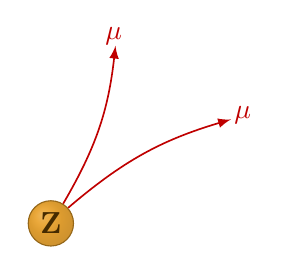
\begin{tikzpicture}[
    scale=2.4, % set scale for all figures
  ]
  
  % Z BOSON
  \node[circle,part=myorange,inner sep=1.8pt,scale=1.1]
    (Z) at (0,0) {\textbf{Z}};
  
  % MUONS
  \draw[track] (Z) to[bend right=12] (70:1.0)
    node[anchor=-80,inner sep=0pt] {$\mu$}; %^-
  \draw[track] (Z) to[bend left=12] (30:1.1)
    node[anchor=-160,inner sep=1pt] {$\mu$}; %^+
  
\end{tikzpicture}


% TAU JET - THREE PRONG, PI ZERO\small
\def\angiso{45} % opening angle of isolation cone (CMS: DR = 0.4 => 0.8*180/pi = 45.8)
\def\angsig{12} % opening angle of signal cone (CMS: 0.05 <= DR <= 0.1 => 0.1*180/pi = 11.4)
\def\e{0.11}    % a/b ratio of ellipse minor and major radii
\begin{tikzpicture}[
    scale=2.4, % set scale for all figures
    every node/.style={inner sep=1,circle} %,draw=black!9,very thin}
  ]
  
  % Z BOSON
  \node[part=myorange,inner sep=1.8pt,scale=1.1]
    (Z) at (0,0) {\textbf{Z}};
  
  % TAUS
  \node[part=mygreen,minimum size=8pt,scale=0.7]
    (T1) at (50:0.3) {};
  \node[part=mygreen,minimum size=8pt,scale=0.7]
    (T2) at (-20:0.3) {};
  \node[mygreen!80!black,anchor=-50,inner sep=1pt,scale=0.9]
    at (T1) {$\tau^+$};
  \node[mygreen!80!black,anchor=60,inner sep=1pt,scale=0.9]
    at (T2) {$\tau^-$};
  \draw[mysmallarrow] (Z) -- (T1);
  \draw[mysmallarrow] (Z) -- (T2);
  
  % MUONS
  \draw[track] (T1) to[out=20,in=-138] ++(32:1.22)
    node[anchor=-160,inner sep=0pt] {$\mu^+$};
  
  % NEUTRINOS
  \begin{scope}[dashed track,opacity=0.4,thin]
    \draw
      (T1) --++ (80:0.64)
      node[anchor=-110,inner sep=0pt,scale=0.8] {$\overline{\nu}_\tau$};
    \draw
      (T1) --++ (50:0.84)
      node[anchor=-150,inner sep=0pt,scale=0.8] {$\nu_\mu$};
    \draw
      (T2) --++ (-29:0.84)
      node[anchor=160,inner sep=1pt,scale=0.8] {$\nu_\tau$};
  \end{scope}
  
  % TAUH
  \begin{scope}[rotate around={-85:(T2)}]
    \coordinate (T2') at ($(T2)+(0,1pt)$); % isolation cone
    \coordinate (I) at ($(T2)+(0,0.92)$); % isolation cone
    \coordinate (S) at ($(T2)+(0,1.00)$); % signal cone
    \coordinate (T) at ($(T2')+(0,0.02)$); % tau vertex
    %\jetcone[isocol]{T2'}{I}{\angiso}{\e}{ % isolation cone
      \jetcone[sigcol]{T2'}{S}{\angsig}{\e}{ % signal cone
        \draw[dashed track] (T) --++ (92:1.18);
          %node[anchor=-85+\anang,inner sep=0.5] {$\pi^0$};
        \draw[track] (T) to[out=90,in=-55] ++(100:1.18);
          %node[anchor=-70+\anang,inner sep={2.5*cos(\ang)^2-1.5}] {$\pi^-$};
        \draw[track] (T) to[out=93,in=-110] ++(85:1.26);
          %node[anchor=-110+\anang,inner sep={0.6*sin(\ang)^2}] {$\pi^+$};
        \draw[track] (T) to[out=88,in=-117] ++(83:1.11);
          %node[anchor=-145+\anang,inner sep={0.6*sin(\ang)^2}] {$\pi^+$};
      }
    %}
    \node[myblue!80!black,anchor=-140,inner sep=0pt]
      at ($(T2)+(0,1.3)$) {$\tau_\mathrm{h}$};
  \end{scope}
  
\end{tikzpicture}


\end{document}